\documentclass{article}

\usepackage{arxiv}

\usepackage[utf8]{inputenc} % allow utf-8 input
\usepackage[T1]{fontenc}    % use 8-bit T1 fonts
\usepackage[hidelinks]{hyperref}       % hyperlinks
\usepackage{url}            % simple URL typesetting
\usepackage{booktabs}       % professional-quality tables
\usepackage{amsmath,amssymb,amsthm}
\usepackage{amsfonts}       % blackboard math symbols
\usepackage{float}
\usepackage{nicefrac}       % compact symbols for 1/2, etc.
\usepackage{microtype}      % microtypography
\usepackage{mathrsfs}
\usepackage{graphicx}
\usepackage{doi}
\usepackage{acronym}
\usepackage{listings}
\usepackage{tikz}
\usepackage[dvipsnames]{xcolor}

\usetikzlibrary{trees}

\newacro{abm}[ABM]{Agent-Based Model}
\newacro{cabm}[CABM]{Cellular Agent-Based Model}
\newacro{ca}[CA]{Cellular Automaton}
\newacroplural{ca}[CA]{Cellular Automata}

\newcommand{\todo}[1]{\colorbox{WildStrawberry}{\textcolor{white}{#1}}}

\title{Bayesian Optimization for parameter estimation of Cell-Based Agent-Based Models}

%\date{September 9, 1985}	% Here you can change the date presented in the paper title
%\date{} 					% Or removing it

\author{
    \href{https://orcid.org/0009-0001-0613-7978}{
        
\includegraphics[scale=0.06]{orcid.pdf}
        \hspace{1mm}Jonas Pleyer
    }
    \thanks{
        \href{https://jonas.pleyer.org}{jonas.pleyer.org},
        \href{https://cellular-raza.com}{cellular-raza.com}
    }\\
	Freiburg Center for Data-Analysis and Modeling\\
	University of Freiburg\\
	\texttt{jonas.pleyer@fdm.uni-freiburg.de} \\
	%% examples of more authors
	\And
    Polina Gaindrik\\
	Freiburg Center for Data-Analysis and Modeling\\
	University of Freiburg\\
	\And
	\href{https://orcid.org/0000-0002-6371-4495}{
        
\includegraphics[scale=0.06]{orcid.pdf}
        \hspace{1mm}Christian Fleck
    }\\
	Freiburg Center for Data-Analysis and Modeling\\
	University of Freiburg
}

% Uncomment to remove the date
%\date{}

% Uncomment to override  the `A preprint' in the header
\renewcommand{\headeright}{Preprint}
%\renewcommand{\undertitle}{Technical Report}
\renewcommand{\shorttitle}{
    Bayesian Optimization for parameter estimation of Cell-Based Agent-Based Models
}

\usepackage{enumitem}
\setlist{nolistsep}

%%% Add PDF metadata to help others organize their library
%%% Once the PDF is generated, you can check the metadata with
%%% $ pdfinfo template.pdf
\hypersetup{
pdftitle={Mathematical Foundations of Cellular Agent-Based Models},
pdfsubject={q-bio.NC, q-bio.QM},
pdfauthor={Jonas Pleyer, Christian Fleck},
pdfkeywords={},
}

% Define definition, example, lemma, proof and theorem.
\newtheorem{definition}{Definition}[section]
\newtheorem{example}[definition]{Example}
\newtheorem{lemma}[definition]{Lemma}
\newtheorem{corollary}[definition]{Corollary}
\newtheorem{theorem}[definition]{Theorem}

% Change numbering of equations
% \numberwithin{equation}{section}

% MAKE TITLES IN THEOREMS BOLD
\makeatletter
\def\th@plain{%
  \thm@notefont{}% same as heading font
  \itshape % body font
}
\def\th@definition{%
  \thm@notefont{}% same as heading font
  \normalfont % body font
}
\makeatother

\begin{document}
\maketitle

%###################################################################################################
\begin{abstract}
\end{abstract}


% keywords can be removed
\keywords{Agent-Based \and Biology \and Bayesian Optimization}

%###################################################################################################
\section{Introduction}
\label{section:introduction}
First notion of bayesian optimization~\cite{Kushner1964}, then in~\cite{Mockus1978}.

Mention AI and hyperparameter-tuning

\subsubsection*{Bayesian Optimization}
\begin{itemize}
    \item Requires less function evaluations
    \item Can optimize nonlinear functions
\end{itemize}

%###################################################################################################
\section{Target System}
\label{section:target-system}
\begin{itemize}
    \item Make clear that black-box optimization is required
    \item Should have some application for real-world scenarios
\end{itemize}

%---------------------------------------------------------------------------------------------------
\subsection{Bacterial Rods}
\label{subsection:bacterial-rods}
\begin{itemize}
    \item Optimize parameters of indidivual agents; fit to data
    \item Fit agents via positions
    \item Fit agents via image comparison (see \texttt{cr\_mech\_coli})
    \item neighbor interaction $\rightarrow$ not diff.-able
\end{itemize}

\begin{figure}[H]
    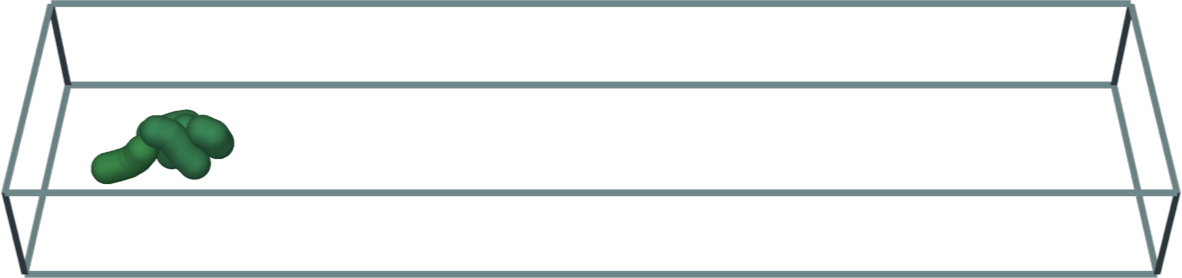
\includegraphics[width=0.48\textwidth]{figures/bacterial-rods-0000000025.png}%
    \hspace{0.04\textwidth}%
    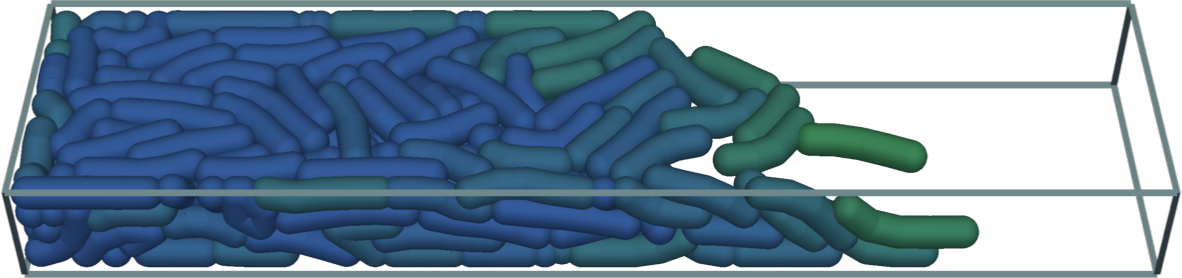
\includegraphics[width=0.48\textwidth]{figures/bacterial-rods-0000007200.png}%
    \caption{\todo{caption}}
    \label{fig:bacterial-rods-sim}
\end{figure}

%---------------------------------------------------------------------------------------------------
\subsection{Bacterial Branching}
\label{subsection:bacterial-branching}
\begin{itemize}
    \item Sensitivity analysis
    \item Calculate fractal dimension of branching pattern
    \item Calculate sensitivity of system with respect to parameters
\end{itemize}

\begin{figure}[H]
    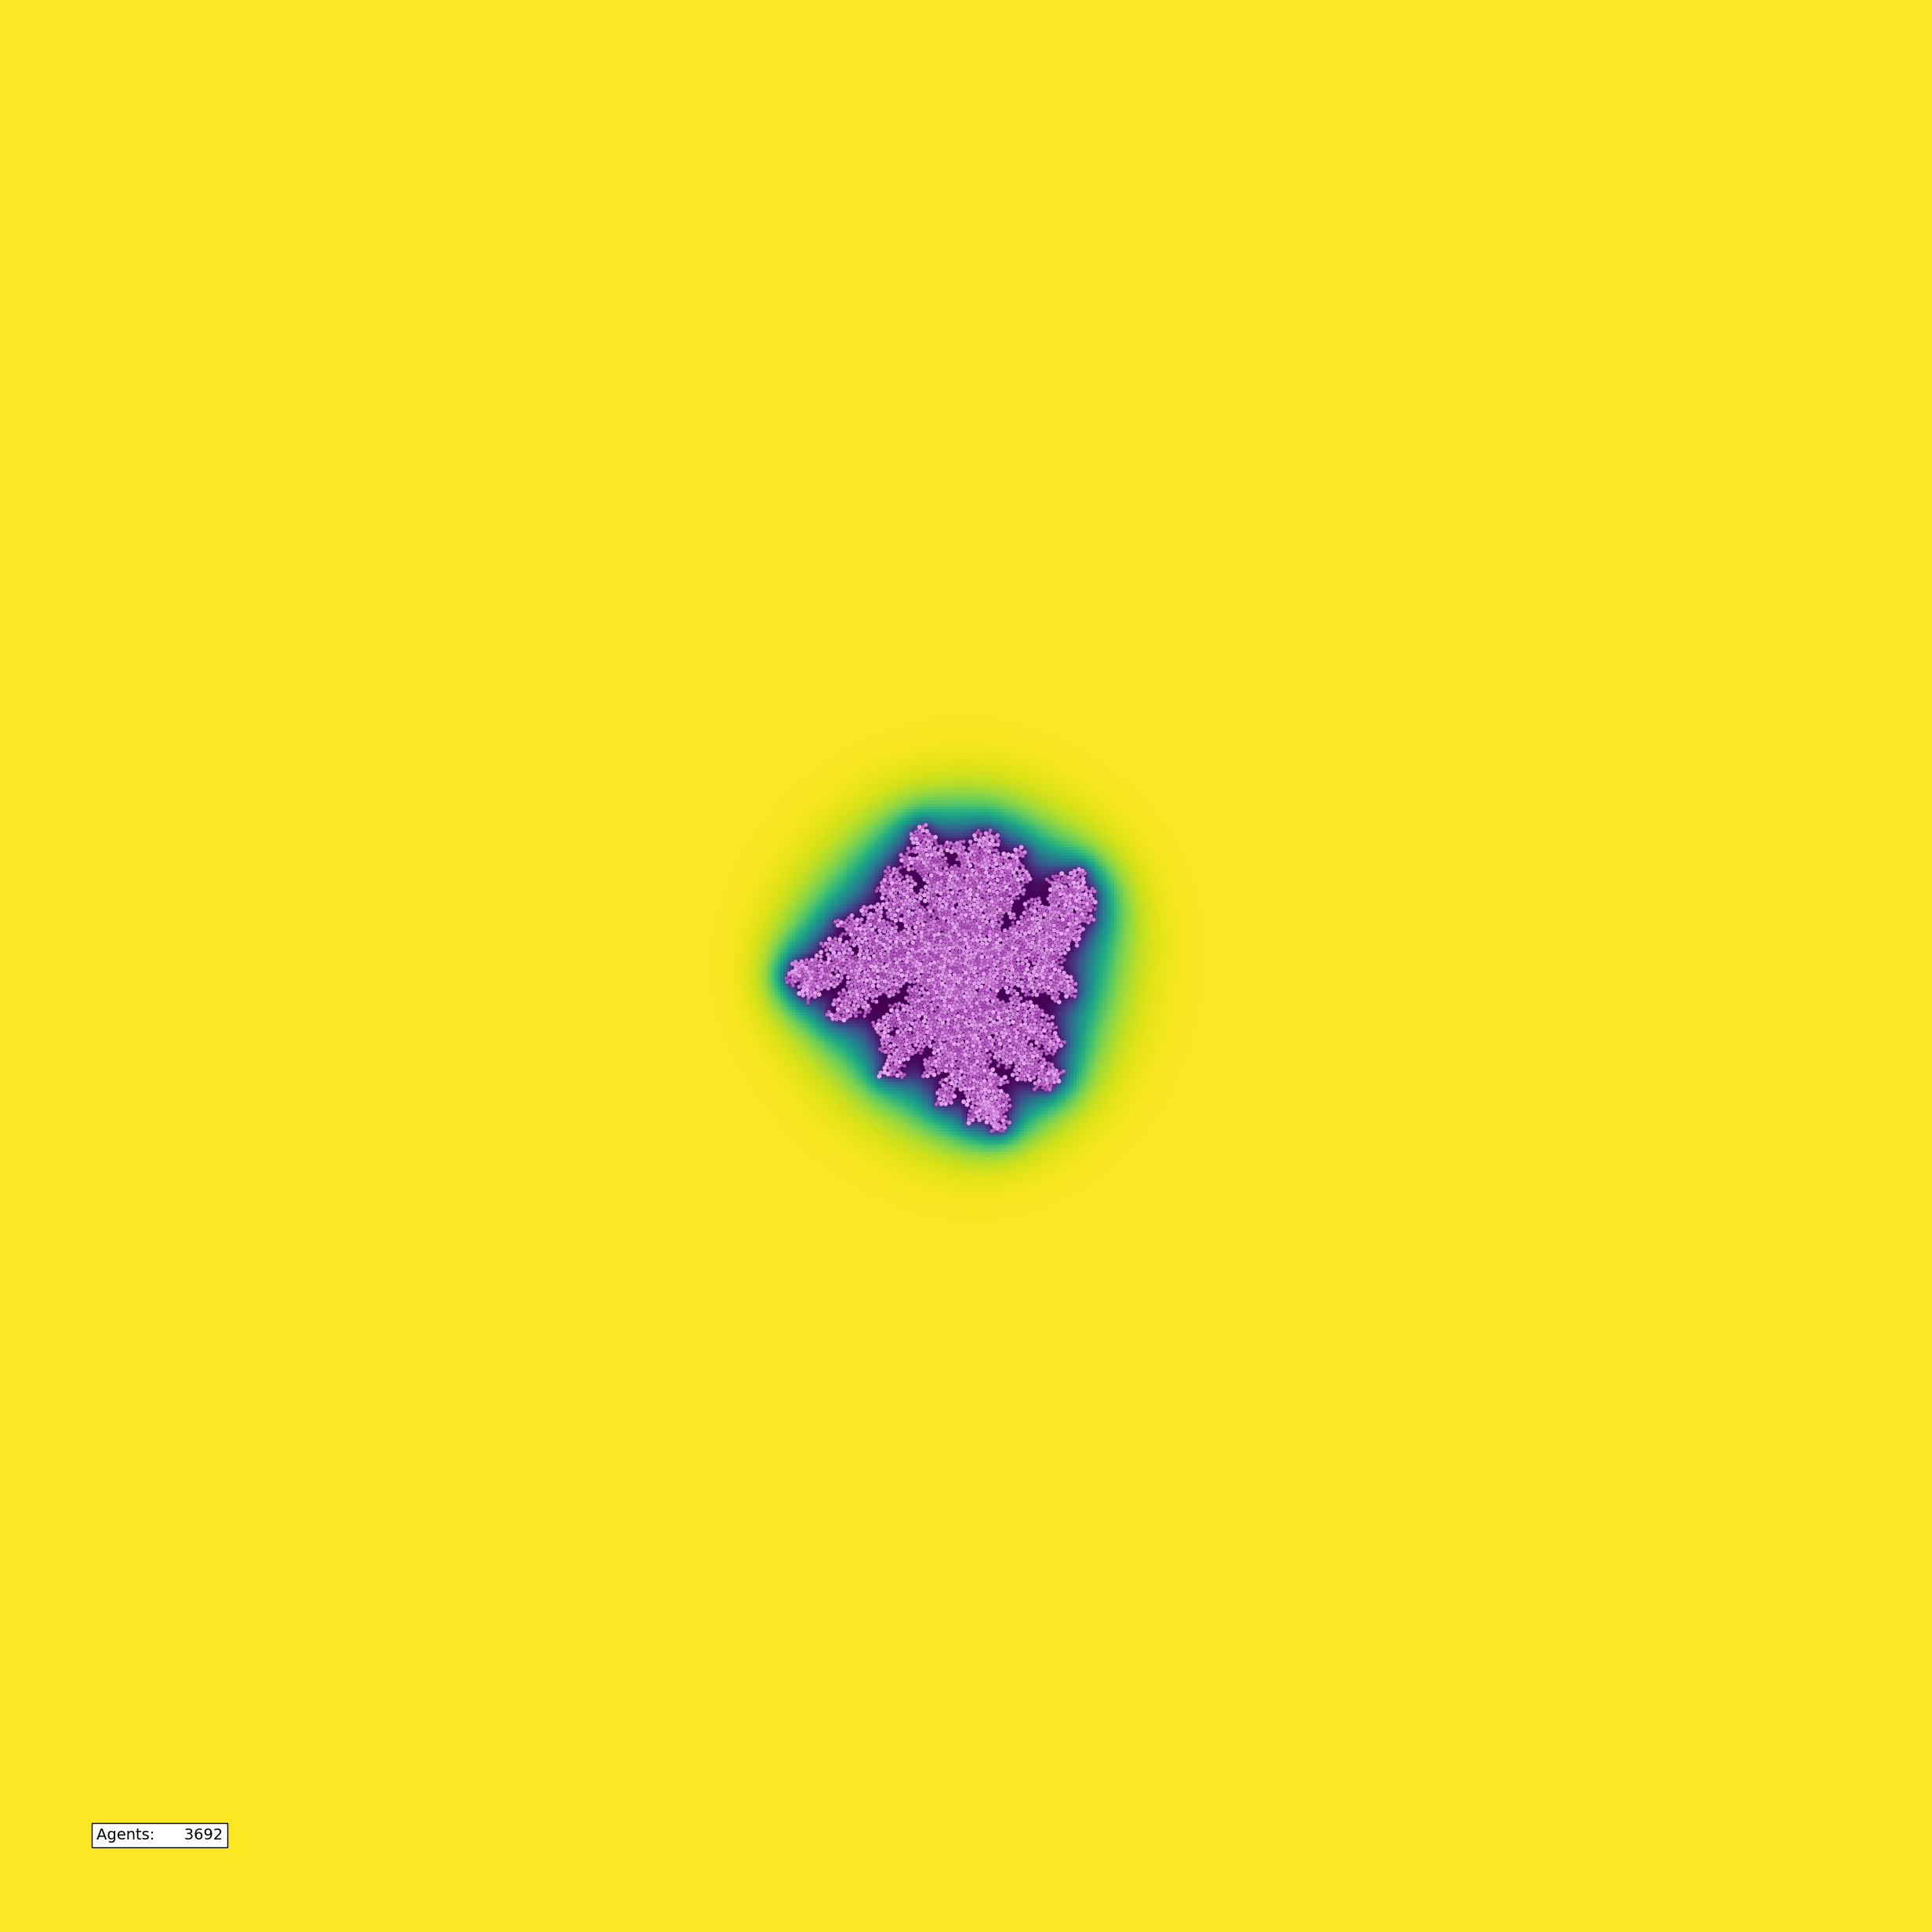
\includegraphics[width=0.48\textwidth]{figures/cells_at_iter_0000009800.png}%
    \hspace{0.04\textwidth}%
    \includegraphics[width=0.48\textwidth]{figures/cells_at_iter_0000060200.png}%
    \caption{\todo{caption}}
    \label{fig:bacterial-branching-sim}
\end{figure}

%###################################################################################################
\section{Optimization}
\label{section:optimization}

Problems of form
\begin{equation}
    \text{max}_{x\in X} f(x)
\end{equation}

\begin{enumerate}
    \item need prior
    \item evaluate $f(x_i)$ for $x_i\in\text{prior}$
    \item form posterior distribution 
    \item construct acquisition function ("infill sampling criteria"); determines next query point
\end{enumerate}

Two methods for defining prior/posterior distributions
\begin{enumerate}
    \item "kriging"
    \item "Parzen-Tree Estimator"
\end{enumerate}

Main citation: \cite{Jones1998}
\begin{itemize}
    \item $f(x)$ difficult to evaluate
    \item $f(x)$ continuous
    \item no derivatives are evaluated
\end{itemize}

%---------------------------------------------------------------------------------------------------
\subsection{Acquisition Functions}
\begin{itemize}
    \item Probability of Improvement
    \item Expected Improvement
    \item Bayesian Expected Losses
    \item Upper Confidence Bounds (UCB) or Lower Confidence Bounds (LCB)
    \item Thompson Sampling
\end{itemize}
Combinations of these are also possible.
All of them are trade-offs between exploration and exploitation to minimize the evaluations of
$f(x)$.

%###################################################################################################
\section{Results}
\label{section:results}

%###################################################################################################
\section{Discussion}
\label{subsection:discussion}

\bibliographystyle{IEEEtran}
\bibliography{references}

%###################################################################################################
\section{Supplementary Material}
\label{section:supplementary-material}

%---------------------------------------------------------------------------------------------------
\subsection{Example}
\label{subsection:supplement-example}

\end{document}
